\documentclass[aspectratio=169]{beamer}
\usepackage[square,numbers]{natbib}
\bibliographystyle{apalike}
\title[AU LaTeX theme]{Imagine the joy of creating AU template presentations in LaTeX}
\date[]{\today}
\author[korsgaard@cs.au.dk]{Henrik Korsgaard}
\institute{DEPARTMENT OF COMPUTER SCIENCE} % Type in A
\usetheme{aarhusuniversity}

\begin{document}

\begin{frame}
\maketitle
\end{frame}

\begin{frame}{Outline}
\tableofcontents
\end{frame}

\section{Background}
\begin{frame}{Motivation}
\begin{itemize}
    \item I use \LaTeX\ in most of my work for writing and dissemination.
    \item I need a solid template for my teaching and talks that fit my writing environment(s).
    \item The official Aarhus University PowerPoint template is well-designed and consistent. 
    \item So, I've created a \LaTeX Beamer theme that closely resemble to the official Aarhus University PowerPoint theme.
\end{itemize}
\end{frame}

\begin{frame}{Notable style differences}

\begin{enumerate}
    \item Default black text replaced with the AU dark blue color as default.
    \item Moved author name and email up under title on front page.
    \item Replaced date and author title in footer with slide counter.
    \item Replaced the circle bullet with triangle for itemized lists
\end{enumerate}
\end{frame}

\begin{frame}[AUMagenta]{Disclaimer and credit}
\begin{enumerate}
    \item I'm not a \LaTeX\ or Beamer prodigy, so stuff may break and be structured and designed unidiomatically.
    \item The theme has not been developed in consultation with others at AU.
    \item This work is inspired by the existing AU Latex templates (see https://medarbejdere.au.dk/en/administration/communication/guidelines/design/latextemplates/)
    \item Questions and comments can be submitted to \insertshortauthor\ or the Gitlab.au.dk repository.
\end{enumerate}
\end{frame}

\section{Download and use}
\begin{frame}[fragile,AUClean]{Download and use}
\begin{enumerate}
    \item Download https://gitlab.au.dk/henrikkorsgaard/au-beamer-template
    \item Locate your Latex TEXMFLOCAL directory\footnotemark
    \item copy the beamerthemeaarhusuniversity.sty into  <TEXMFLOCAL path>/texmf/tex/latex/beamer-aarhusuniversity/
    \item update latex package index with \verb=sudo texhash=
    \item Download and install the AU font globally on your system
    \item Set document class \verb=\documentclass[aspectratio=169]{beamer}=
    \item Set theme \verb=\usetheme{aarhusuniversity}=
\end{enumerate}
\footnotetext{See https://gitlab.au.dk/henrikkorsgaard/au-beamer-template/README.md or https://jeffreywong.ca/tutorials/installing-a-custom-beamer-theme-latex/ for more information}
\end{frame}

\begin{frame}[fragile,AUClean]{Using with Overleaf}
\begin{enumerate}
    \item Download https://gitlab.au.dk/henrikkorsgaard/au-beamer-template
    \item Unzip and upload to Overleaf project
    \item Set the latex compiler to xelatex in the menu
    \item Set document class \verb=\documentclass[aspectratio=169]{beamer}=
    \item Set theme \verb=\usetheme{aarhusuniversity}=
\end{enumerate}
\end{frame}

\section{Basic design and features}
\begin{frame}[fragile]{Generating the title page}%here fragile is necessary in order to use the \verbatim environment
\begin{description}[Institution]
\item[Title] \verb=\title[short]{full}= sets the presentation title. `Full' is for the main title page. `Short' title is inserted in the running footer. 
\item[Author] \verb=\author[email]{name}= sets the presentation author. `Name' is the full author name. `Email' is reserved for contact email on the title page.
\item[Date] \verb=\date{date}= inserts the date in the title page footer. This field can also be used for, e.g. location or event information.
\item[Institution] \verb=\institute{department}= inserts the department name under the AU logo in the footer.
\end{description}
\end{frame}

\begin{frame}[fragile]{Creating frames}%here fragile is necessary in order to use the \verbatim environment
\begin{columns}
\begin{column}{0.5\textwidth}
   \begin{itemize}
        \item The \verb=\begin{frame}= command creates the frame environment, see full example to the right.
       \item Options are for setting frame labels or template specific frame types -- see next slide and the examples section 
       \item Examine the main.tex file and Beamer class for more \LaTeX\ code examples
    \end{itemize}
\end{column}
\begin{column}{0.45\textwidth}  %%<--- here
    \verb=\begin{frame}[options]{title}=\\
        \hspace{1em}\dots content \dots\\
    \verb=\end{frame}=
\end{column}
\end{columns}
\end{frame}

\begin{frame}[AUDark]{Frame style [options]}
\begin{description}[AUCleanDark]
\item[AUDark] generates a frame with a dark blue background and white text similar to this slide.
\item[AUGreen] generates a frame with a green background and white text.
\item[AUMagenta] generates a frame with a magenta background and white text.
\item[AUClean] generates a frame without a footer.
\item[AUDarkClean] generates a frame with a dark blue background and without a footer.
\end{description}
\end{frame}

\begin{frame}[fragile, AUClean]{Fonts and logos}
\begin{description}
\item[Regular] This is the normal AU Passata font
\item[Bold]  \verb=\textbf= \textbf{For AU Passata Bold}
\item[Italics] \verb=\textit= or \verb=\emph= \textit{For AU Passata Regular Oblique}
\item[Light] \verb=\textlight= \textlight{For AU Passata Light}
\item[Peto] \verb=\peto= \peto{For AU Peto}\footnotemark
\item[AU Seal] \verb=\AUSeal= \hspace{0.5em}\AUSeal\hspace{0.5em}(use fontsize to change)\footnotemark[\value{footnote}]
\item[AU Logo] \verb=\AULogo= \hspace{0.5em}\AULogo\hspace{0.5em}(use fontsize to change)\footnotemark[\value{footnote}]
\item[AU BSS Logo] \verb=\BSSLogo= \hspace{0.5em}\BSSLogo \hspace{0.5em} (use fontsize to change)\footnotemark[\value{footnote}]
\end{description}
\footnotetext{These font features currently do not work on the Overleaf variant}
\end{frame}

\section{Examples}

\begin{frame}[fragile]{Columns}
\begin{columns}
\begin{column}{0.45\textwidth}
   It is very easy to make a two-column design for a slide, e.g. for inserting additional text, images, quotes or examples in the right-hand column.\\
   \vspace{1em}
   The right-hand example illustrates how to do this with the columns environment. A column width of \verb=0.45\textwidth= fit the template.
\end{column}
\begin{column}{0.45\textwidth}
    \verb=\begin{columns}=\\
        \hspace{1em}\verb=\begin{column}{width}=\\
        \hspace{2em}\dots content \dots\\
        \hspace{1em}\verb=\end{column}=
        \hspace{1em}\verb=\begin{columns}=\\
        \hspace{1em}\verb=\begin{column}{0.45\textwidth}=\\
        \hspace{2em}\dots content \dots\\
        \hspace{1em}\verb=\end{column}=\\
    \verb=\end{columns}=
\end{column}
\end{columns}
\end{frame}

\begin{frame}{Lists: Enumerate and Itemize}
\begin{columns}
\begin{column}{0.45\textwidth}
    \begin{enumerate}
        \item Enumerated lists
        \item use standard numbering 
        \begin{enumerate}
            \item Lists can be embedded 
            \item just as in \LaTeX
    \end{enumerate}
    \end{enumerate}
\end{column}
\begin{column}{0.45\textwidth}
    \begin{itemize}
        \item Itemized lists
        \item are ideal for bullet content
        \begin{enumerate}
            \item You can mix embedded lists
            \item just as in \LaTeX
        \end{enumerate}
    \end{itemize}
\end{column}
\end{columns}
\end{frame}

\begin{frame}[AUDark]{Lists: Description}
\begin{description}
\item[What] The template support the use of descriptive lists
\item[Why] These are useful for when listing concepts or positions etc.
\item[When] Or to summarize deadlines, multiple slides or other key information.
\end{description}

\end{frame}
\begin{frame}{Images}
\begin{figure}[h]
\centering
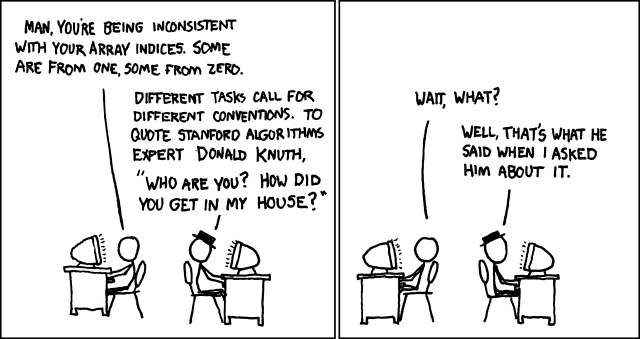
\includegraphics[width=0.7\textwidth]{images/donald_knuth.png}
\caption{XKCD: Donald Knuth (\url{https://xkcd.com/163/})}
\end{figure}
\end{frame}

\begin{frame}{Tables}
\centering
We can make tables just as in \LaTeX\ documents, see e.g. table \ref{tab:cutlery}.
\begin{table}[]
\centering
\begin{tabular}{| c | c | c | c |}
\hline
 \textbf{Location} & \textbf{Forks} & \textbf{Knives} & \textbf{Spoons} \\ 
 \hline
 In drawer & 6 & 87837 & 787 \\ 
  \hline
 In use & 7 & 78 & 5415 \\
  \hline
 In the dishwasher & 545 & 778 & 7507 \\
 \hline
\end{tabular}
\caption{Cutlery overview}
\label{tab:cutlery}
\end{table}   
\end{frame}

\begin{frame}[fragile]{References}
\begin{columns}
\begin{column}{0.5\textwidth}
We can use citations as usual using \verb=\cite{<key>}= with style options from the \verb=natbib= package.\\
\vspace{0.5em}
When using citations, e.g. \cite{tantau2004user, mertz2005beamer}, we need to generate the reference list in a frame somewhere \verb=\bibliography{<bib file>}= command.
\end{column}
\begin{column}{0.45\textwidth}
Example of the bibligraphy list\\
\vspace{1em}
\bibliography{references}
\vspace{1em}
Note, that with long reference lists, it is necessary to add the \verb=allowframebreaks= to the frame option list.
\end{column}
\end{columns}
\end{frame}

\begin{frame}[fragile]{Math}
    \begin{columns}
    \begin{column}{0.45\textwidth}
       Per request formula in a math environment uses the Computer Modern font (cmr) and the color black on white slides. For other slides the color is likely white. 
    \end{column}
    \begin{column}{0.45\textwidth}
        \Huge
        \centering
        \begin{math}
            \Delta U = Q - W
        \end{math}
    \end{column}
    \end{columns}
    \end{frame}

\begin{frame}[AUDark]{Example of the [AUDark] slide option}
\end{frame}

\begin{frame}[AUGreen]{Example of the [AUGreen] slide option}
\end{frame}

\begin{frame}[AUMagenta]{Example of the [AUMagenta] slide option}
\end{frame}

\begin{frame}[AUClean]{Example of the [AUClean] slide option}
\centering
If you omit the slide title, it will be empty as well!
\end{frame}

\begin{frame}[AUDarkClean]{}
\centering
\huge Example of the [AUDarkClean] slide option without footer and in this case and empty title
\end{frame}

\section{Final notes}
\begin{frame}[fragile]{Known Issues}
    \begin{itemize}
        \item The command \verb=\insertinstitute= do not cooperate with \verb=\MakeUppercase=. Hence, \verb=\institute{department}= does not auto capitalize the department name. This needs to be done manually.
        \item The \verb=\begin{description}= list is a bit sensitive to long descriptors. Consider just using a item list instead.
    \end{itemize}
\end{frame}

\begin{frame}[AUDark]{Feedback}
    \begin{itemize}
        \item Write \insertauthor\ at \insertshortauthor\\
        \item Post an issue on https://gitlab.au.dk/henrikkorsgaard/au-beamer-template
    \end{itemize}
\end{frame}

\end{document}